\section{High energy physics research at the CMS 
     experiment at the Large Hadron Collider}


At the heart of CMS is the silicon pixel detector that provides three
high-precision space point measurements to reconstruct charged
particle trajectories. These three points are sufficient to produce
good track information for the High Level Trigger (HLT) and for the
efficient seeding of track reconstruction in the full tracker
volume. The close proximity of the first detector layer to the
interaction point (4.4 cm) minimizes multiple scattering effects and
extrapolation uncertainties making the pixel information crucial for
the reconstruction of the initial position and direction of the
charged tracks. The pixel detector therefore plays a key role in the
identification of primary vertices, secondary vertices, and secondary
tracks. These elements are essential for the efficient identification
of long-lived particles, such as b quarks, and for the search for new
physics at the LHC.

\begin{figure}[htb]
  \centering
  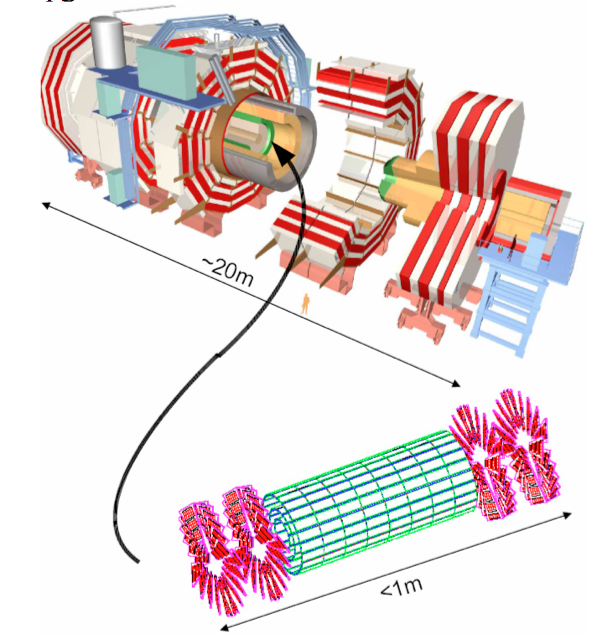
\includegraphics[width=0.5\textwidth]{CMS_detector_low_res.png}
  \caption{\label{fig:cms}
    A diagram of the CMS experiment and the pixel portion of the
    tracking detector.
  }
\end{figure}
